\textbf{{异步通信}}没有公共的时钟标准,不要求所有部件严格地统一操作时间,而是采用\textbf{应答的方式(或称握手方式)},即当主模块发出请求信号时,一直等待从模块反馈``响应''信号后才开始通信。当然,这就要求主、从模块之间增加两条应答线。

异步通信的应答方式又可分为\textbf{不互锁、半互锁和全互锁}3种类型,如下图所示。

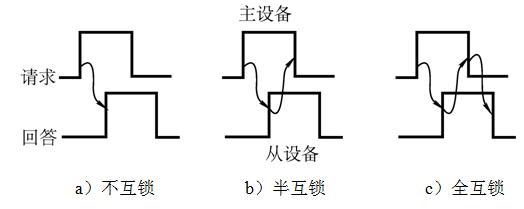
\includegraphics[width=3.33333in,height=1.33333in]{png-jpeg-pics/AE32CB814F07430268B0F6C028FF34B7.png}

{\textbf{1. 不互锁方式}}

特点:主模块的请求信号和从模块的回答信号没有互相的制约关系。

\textbf{{2. 半互锁方式}}

特点:主模块的请求信号和从模块的回答信号有简单的制约关系。

{\textbf{3. 全互锁方式}}

特点:主模块的请求信号和从模块的回答信号有完全的制约关系。
